\documentclass{article}

\usepackage{fancyhdr}
\usepackage{extramarks}
\usepackage{amsmath}
\usepackage{amsthm}
\usepackage{amssymb}
\usepackage{amsfonts}
\usepackage{tikz}
\usepackage{physics}
\usepackage[plain]{algorithm}
\usepackage{algpseudocode}
\usepackage{graphicx,wrapfig,lipsum}
\usetikzlibrary{automata,positioning}

%
% Basic Document Settings
%

\topmargin=-0.45in
\evensidemargin=0in
\oddsidemargin=0in
\textwidth=6.5in
\textheight=9.0in
\headsep=0.25in

\linespread{1.1}

\pagestyle{fancy}
\lhead{\hmwkAuthorName}
\chead{\hmwkClass\ : \hmwkTitle}
\rhead{\firstxmark}
\lfoot{\lastxmark}
\cfoot{\thepage}

\renewcommand\headrulewidth{0.4pt}
\renewcommand\footrulewidth{0.4pt}

\setlength\parindent{0pt}

%
% Create Problem Sections
%
\newcommand{\be}{\begin{equation}}
\newcommand{\ee}{\end{equation}}
\newcommand{\bes}{\begin{equation*}}
\newcommand{\ees}{\end{equation*}}
\newcommand{\bea}{\begin{flalign*}}
\newcommand{\eea}{\end{flalign*}}


\newcommand{\enterProblemHeader}[1]{
    \nobreak\extramarks{}{Problem \arabic{#1} continued on next page\ldots}\nobreak{}
    \nobreak\extramarks{Problem \arabic{#1} (continued)}{Problem \arabic{#1} continued on next page\ldots}\nobreak{}
}

\newcommand{\exitProblemHeader}[1]{
    \nobreak\extramarks{Problem \arabic{#1} (continued)}{Problem \arabic{#1} continued on next page\ldots}\nobreak{}
    \stepcounter{#1}
    \nobreak\extramarks{Problem \arabic{#1}}{}\nobreak{}
}

\setcounter{secnumdepth}{0}
\newcounter{partCounter}
\newcounter{homeworkProblemCounter}
\setcounter{homeworkProblemCounter}{1}
\nobreak\extramarks{Problem \arabic{homeworkProblemCounter}}{}\nobreak{}

%
% Homework Problem Environment
%
% This environment takes an optional argument. When given, it will adjust the
% problem counter. This is useful for when the problems given for your
% assignment aren't sequential. See the last 3 problems of this template for an
% example.
%
\newenvironment{homeworkProblem}[1][-1]{
    \ifnum#1>0
        \setcounter{homeworkProblemCounter}{#1}
    \fi
    \section{Problem \arabic{homeworkProblemCounter}}
    \setcounter{partCounter}{1}
    \enterProblemHeader{homeworkProblemCounter}
}{
    \exitProblemHeader{homeworkProblemCounter}
}

%
% Homework Details
%   - Title
%   - Due date
%   - Class
%   - Section/Time
%   - Instructor
%   - Author
%

\newcommand{\hmwkTitle}{Assignment\ \#4}
\newcommand{\hmwkDueDate}{Due on 13th November, 2018}
\newcommand{\hmwkClass}{Fluid Mechanics}
\newcommand{\hmwkClassTime}{}
\newcommand{\hmwkClassInstructor}{}
\newcommand{\hmwkAuthorName}{\textbf{Aditya Vijaykumar}}

%
% Title Page
%

\title{
    %\vspace{2in}
    \textmd{\textbf{\hmwkClass:\ \hmwkTitle}}\\
    \normalsize\vspace{0.1in}\small{\hmwkDueDate\ }\\
%    \vspace{3in}
}

\author{\hmwkAuthorName}
\date{}

\renewcommand{\part}[1]{\textbf{\large Part \Alph{partCounter}}\stepcounter{partCounter}\\}

%
% Various Helper Commands
%

% Useful for algorithms
\newcommand{\alg}[1]{\textsc{\bfseries \footnotesize #1}}

% For derivatives
\newcommand{\deriv}[1]{\frac{\mathrm{d}}{\mathrm{d}x} (#1)}

% For partial derivatives
\newcommand{\pderiv}[2]{\frac{\partial}{\partial #1} (#2)}

% Integral dx
\newcommand{\dx}{\mathrm{d}x}

% Alias for the Solution section header
\newcommand{\solution}{\textbf{\large Solution}}

% Probability commands: Expectation, Variance, Covariance, Bias
\newcommand{\E}{\mathrm{E}}
\newcommand{\Var}{\mathrm{Var}}
\newcommand{\Cov}{\mathrm{Cov}}
\newcommand{\Bias}{\mathrm{Bias}}

\begin{document}

\maketitle
\textbf{Acknowledgements} -





\begin{homeworkProblem}[1]
	In ideal $2$D flow, $ \div{\va{u}} = 0 $. This means,
	\begin{equation*}
	\pdv{u}{x} + \pdv{v}{y} = 0 \implies u = \pdv{\psi}{y} \qq{and} v = - \pdv{\psi}{x}
	\end{equation*}
	Hence, $ \grad{\psi} = \pdv{\psi}{x} \vu{x} + \pdv{\psi}{y} \vu{y} = -v \vu{x} +  u \vu{y} $. By definition $ \va{u} = \grad{\phi} = u \vu{x} + v \vu{y} $. Now we can do the calculations required in the problem,
	
	\begin{itemize}
		\item $ \grad{\psi} \vdot \grad{\phi} = (-v \vu{x} +  u \vu{y})  \vdot  ( u \vu{x} + v \vu{y} ) = -vu + uv = 0$.
		\item $ - \grad{\psi} \cross \grad{\phi} = - (-v \vu{x} +  u \vu{y}) \cross  ( u \vu{x} + v \vu{y} ) =  - (-v^2 - u^2 )\vu{z} = \abs{\va{u}}^2 \vu{z} $
		\item $\abs{\grad{\psi}}^2 = u^2 + v^2 \qq{and}  \abs{\grad{\phi}}^2 = u^2 + v^2 \implies  \abs{\grad{\psi}}^2 = \abs{\grad{\phi}}^2$ 
		\item $ -\vu{z} \cross \grad{\psi} = -\vu{z} \cross (-v \vu{x} +  u \vu{y} ) = u \vu{x} + v \vu{y}  = \grad{\phi} $
	\end{itemize}
\end{homeworkProblem}














\begin{homeworkProblem}[2]
	\begin{itemize}
		\item For point source, $ \va{u} = \dfrac{q_s}{2 \pi r} \vu{r} $, where $ q_s $ is the source strength. In spherical polar coordinates, $  \va{u} = \pdv{\phi}{r} \vu{r} + \frac{1}{r} \pdv{\phi}{\theta} \vu{\theta} $. This means
		\begin{equation*}
		\phi = \int \pdv{\phi}{r} dr + \int \dfrac{1}{r} \pdv{\phi}{\theta} d\theta  = \dfrac{q_s}{2\pi} \ln r + constant
		\end{equation*}
		For lines of constant $ \phi $,
		\begin{align*}
		\dfrac{q_s}{2\pi} \ln r &= C\\
		\implies \dfrac{q_s}{2\pi r} \dv{r}{x} &= 0\\
		\implies \dfrac{q_s}{2\pi r^2} \qty(2x + 2y \dv{y}{x}) &= 0 \implies  \dv{y}{x} = - \dfrac{x}{y} = m
		\end{align*}
		As velocity is radial, the streamlines are also radial straight lines passing through the origin. The slope of such straight lines is $ \dfrac{y}{x} = - \dfrac{1}{m} $. Hence the streamlines and lines of constant $ \psi $ are perpendicular.
		
		\item For point vortex, $ \va{u} = \dfrac{\Gamma}{2 \pi r} \vu{\theta} = \dfrac{ -\Gamma y}{2 \pi (x^2 + y^2)} \vu{x} + \dfrac{ \Gamma x}{2 \pi (x^2 + y^2)} \vu{y} $. This means,
		\begin{equation*}
		\phi =  \dfrac{\Gamma}{2 \pi} \tan^{-1} \dfrac{y}{x} \qq{and} \psi = - \dfrac{\Gamma}{2 \pi} \ln r
		\end{equation*}
		For lines of constant $ \phi $,
		\begin{align*}
		\dfrac{\Gamma}{2 \pi} \tan^{-1} \dfrac{y}{x} &= C_1\\
		\implies \dfrac{y}{x} &= constant = m_1\\
		\implies  \dv{y}{x} &= m_1
		\end{align*}
		For lines of constant $ \psi $,
		\begin{align*}
		\dfrac{\Gamma}{2 \pi} \ln r &= C_2\\
		\implies r &= constant\\
		\implies  x^2 + y^2 &= constant\\
		\implies \dv{y}{x} &= - \dfrac{x}{y} = - \dfrac{1}{m_1}
		\end{align*}
		Hence proved.
	\end{itemize}
	
\end{homeworkProblem}









\begin{homeworkProblem}[3]
	Given $ A =  \mqty[-1 & p \\ 0 & -2] $. The eigenvalues of $ A $ are $ \lambda_1 = -1 $ and $ \lambda_2 = -2 $ with corresponding (normalized) eigenvectors are $v_1 = \mqty[1 & 0]^T$ and $ v_2 = \mqty[\dfrac{-p}{\sqrt{1 + p^2}} & \dfrac{1}{\sqrt{1 + p^2}}]^T $. So, the resultant vector is,
	\begin{align*}
	v &= v_1 e^{\lambda_1 t} + v_2 e^{\lambda_2 t}\\
	&= \mqty[1 \\ 0] e^{-t} + \dfrac{1}{\sqrt{1 +p^2}}\mqty[{-p} \\ {1}] e^{-2t}\\
	v &= \mqty[e^{-t} -\frac{p}{\sqrt{1 + p^2}} e^{-2t} \\ \frac{1}{\sqrt{1 + p^2}} e^{-2t}]\\
	\abs{v}^2 &= \qty(e^{-t} -\frac{p}{\sqrt{1 + p^2}} e^{-2t} )^2 + \qty(\frac{1}{\sqrt{1 + p^2}} e^{-2t})^2\\
	&= e^{-2t} + e^{-4t} - \dfrac{2p}{\sqrt{1 + p^2}} e^{-3t}\\
	\dv{\abs{v}^2}{t} &= -2 e^{-2t} -4 e^{-4t} + \dfrac{6p}{\sqrt{1 + p^2}} e^{-3t}
 	\end{align*}
	For the resultant to grow, $ \dv{\abs{v}^2}{t} > 0 $.
	\begin{align*}
	\implies -2 e^{-2t} -4 e^{-4t} + \dfrac{6p}{\sqrt{1 + p^2}} e^{-3t} &> 0\\
	\implies \dfrac{p}{\sqrt{1 + p^2}} &> \dfrac{ e^{t} + 2 e^{-t}}{3}
	\end{align*}
	The function $ \dfrac{ e^{t} + 2 e^{-t}}{3} $ has a minimum value of $ \dfrac{2\sqrt{2}}{3} $. Hence, for the resultant to grow for some finite time,
	\begin{align*}
	\dfrac{p}{\sqrt{1 + p^2}} &> \dfrac{2 \sqrt{2}}{3}\\
	\implies \dfrac{p^2}{1 + p^2} &> \dfrac{8}{9}\\
	\implies p^2 &> 8 \\
	\implies p &> 2 \sqrt{2}
	\end{align*}
	Hence, the resultant will grow for some finite time if $ p > 2 \sqrt{2} $.
	
\end{homeworkProblem}












\begin{homeworkProblem}[4]
	\begin{figure}[h!]
		\centering
		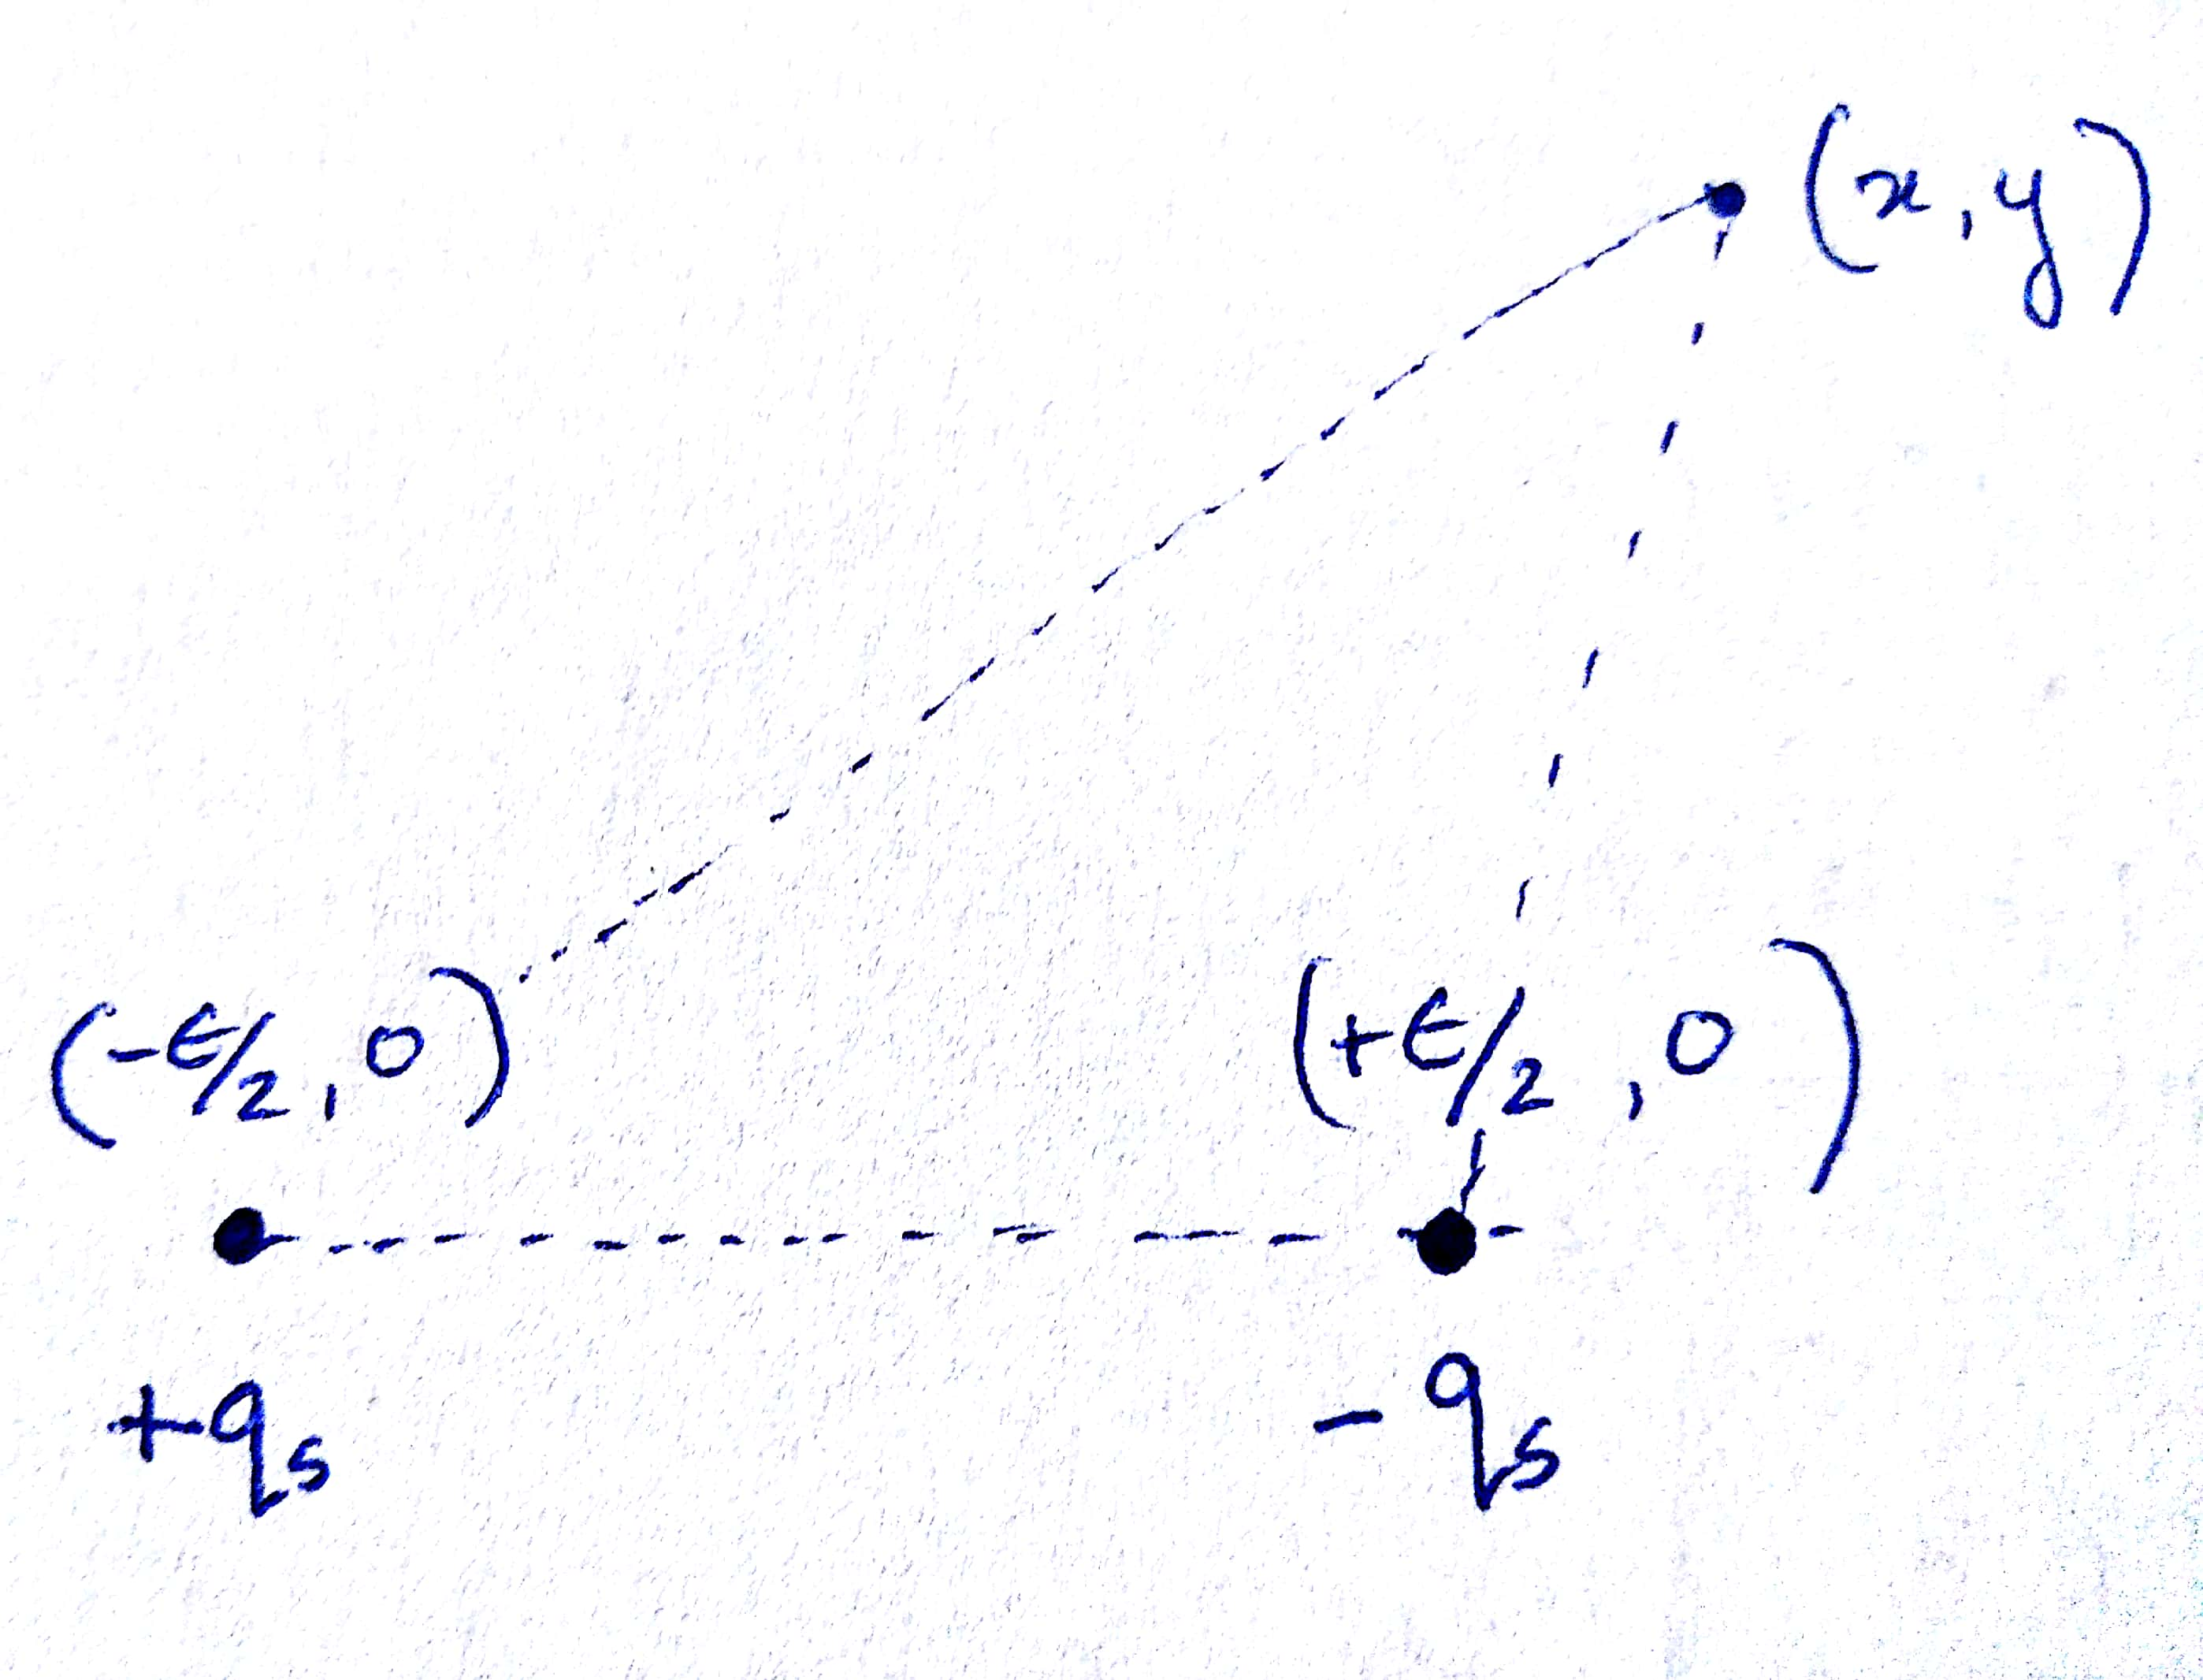
\includegraphics[scale=0.09]{q2.jpg}
	\end{figure}
	Let's first find the potential. As described in Problem 1, $ \phi = \dfrac{q_s}{2 \pi} \ln r $. So for this problem,
	\begin{align*}
	\phi &= -\dfrac{q_s}{4 \pi} \ln [(x - \epsilon/2)^2 + y^2] + \dfrac{q_s}{4 \pi} \ln [(x + \epsilon/2)^2 + y^2] \\
	&= \dfrac{q_s}{4 \pi} \ln \dfrac{(x + \epsilon/2)^2 + y^2}{(x - \epsilon/2)^2 + y^2}\\
	&= \dfrac{q_s}{4 \pi} \ln \dfrac{1 + \epsilon x / r^2 }{1 - \epsilon x /r^2 }\\
	&= \dfrac{q_s}{4 \pi} \ln ({1 + 2\epsilon x / r^2 })\\
	\phi &= \dfrac{q_s \epsilon \cos \theta}{2 \pi r}
	\end{align*}
	
	Hence, the velocity profile is,
	\begin{equation*}
	\va{u} = -\dfrac{q_s \epsilon \cos \theta}{2 \pi r^2} \vu{r} - \dfrac{q_s \epsilon \sin \theta}{2 \pi r^2} \vu{\theta}
	\end{equation*}
	For the streamlines, we note that for a single point source at origin, \begin{align*}
	u = \dfrac{q_s x}{2 \pi (x^2 + y^2)} &\qq{and} v = \dfrac{q_s y}{2 \pi (x^2 + y^2)}\\
	\therefore \psi &= \dfrac{q_s}{2 \pi} \tan^{-1} \dfrac{y}{x}
	\end{align*}
	Hence, for this problem,
	\begin{align*}
	\psi &= -\dfrac{q_s}{2 \pi} \tan^{-1} \dfrac{y}{x - \epsilon/2} + \dfrac{q_s}{2 \pi} \tan^{-1} \dfrac{y}{x + \epsilon/2}\\
	&= \dfrac{q_s}{2 \pi} \qty(\tan^{-1} \dfrac{y}{x + \epsilon/2} - \tan^{-1} \dfrac{y}{x - \epsilon/2} )\\
	&= \dfrac{q_s}{2 \pi} \tan^{-1} \dfrac{y(x - \epsilon/2 - x - \epsilon/2) }{x^2 + y^2}\\
	&= \dfrac{q_s}{2 \pi} \tan^{-1} \dfrac{-y\epsilon}{r^2}\\
	\psi &= - \dfrac{q_s}{2 \pi} \dfrac{\sin \theta}{r}
	\end{align*}
	
	\begin{equation*}
	\psi = - \dfrac{q_s}{2 \pi} \dfrac{\sin \theta}{r} = constant \implies \dfrac{\sin \theta}{r } = \dfrac{y}{x^2 + y^2} = \dfrac{1}{2C} \implies x^2 + (y - C)^2 = C^2
	\end{equation*}
	which is the equation of a circle with centre at $ (0,C) $ and radius $ C $.
\end{homeworkProblem}

\end{document}
